\documentclass{standalone}
\usepackage{tikz}
\usetikzlibrary{patterns, positioning}

\begin{document}
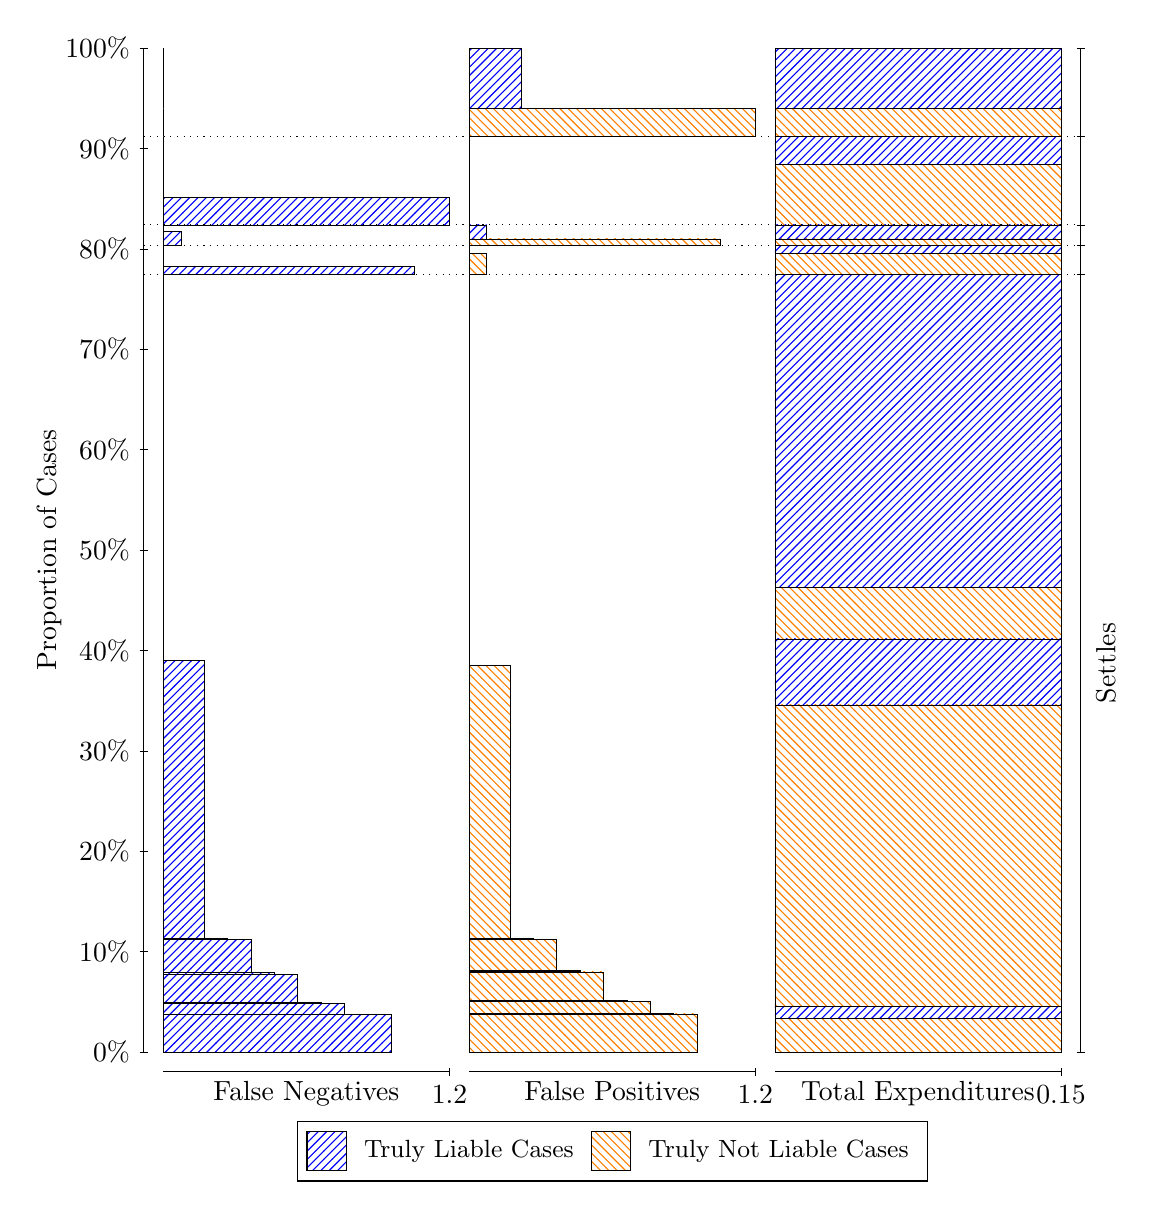
\begin{tikzpicture}
\draw[black, very thin] (1.5,1.75) -- (1.5,14.5);
\node[rotate=90, anchor=center] at (0.3, 8.125) {Proportion of Cases};
\draw[black, very thin] (1.45,1.75) -- (1.55,1.75);
\node[anchor=east] at (1.45, 1.75) {0\%};
\draw[black, very thin] (1.45,3.025) -- (1.55,3.025);
\node[anchor=east] at (1.45, 3.025) {10\%};
\draw[black, very thin] (1.45,4.3) -- (1.55,4.3);
\node[anchor=east] at (1.45, 4.3) {20\%};
\draw[black, very thin] (1.45,5.575) -- (1.55,5.575);
\node[anchor=east] at (1.45, 5.575) {30\%};
\draw[black, very thin] (1.45,6.85) -- (1.55,6.85);
\node[anchor=east] at (1.45, 6.85) {40\%};
\draw[black, very thin] (1.45,8.125) -- (1.55,8.125);
\node[anchor=east] at (1.45, 8.125) {50\%};
\draw[black, very thin] (1.45,9.4) -- (1.55,9.4);
\node[anchor=east] at (1.45, 9.4) {60\%};
\draw[black, very thin] (1.45,10.675) -- (1.55,10.675);
\node[anchor=east] at (1.45, 10.675) {70\%};
\draw[black, very thin] (1.45,11.95) -- (1.55,11.95);
\node[anchor=east] at (1.45, 11.95) {80\%};
\draw[black, very thin] (1.45,13.225) -- (1.55,13.225);
\node[anchor=east] at (1.45, 13.225) {90\%};
\draw[black, very thin] (1.45,14.5) -- (1.55,14.5);
\node[anchor=east] at (1.45, 14.5) {100\%};

\draw[black, very thin] (13.4,1.75) -- (13.4,14.5);
\draw[black, very thin] (13.35,1.75) -- (13.45,1.75);
\node[anchor=west] at (13.35, 1.75) {};
\draw[black, very thin] (13.35,11.629) -- (13.45,11.629);
\node[anchor=west] at (13.35, 11.629) {};
\draw[black, very thin] (13.35,11.991) -- (13.45,11.991);
\node[anchor=west] at (13.35, 11.991) {};
\draw[black, very thin] (13.35,12.255) -- (13.45,12.255);
\node[anchor=west] at (13.35, 12.255) {};
\draw[black, very thin] (13.35,13.377) -- (13.45,13.377);
\node[anchor=west] at (13.35, 13.377) {};
\draw[black, very thin] (13.35,14.5) -- (13.45,14.5);
\node[anchor=west] at (13.35, 14.5) {};

\draw[black, very thin, pattern color=blue, pattern=north east lines] (1.75,1.75) rectangle (4.6418,2.2232);
\draw[black, very thin, pattern color=blue, pattern=north east lines] (1.75,2.2232) rectangle (4.3452,2.2273);
\draw[black, very thin, pattern color=blue, pattern=north east lines] (1.75,2.2273) rectangle (4.0486,2.3679);
\draw[black, very thin, pattern color=blue, pattern=north east lines] (1.75,2.3679) rectangle (3.752,2.3757);
\draw[black, very thin, pattern color=blue, pattern=north east lines] (1.75,2.3757) rectangle (3.4554,2.7399);
\draw[black, very thin, pattern color=blue, pattern=north east lines] (1.75,2.7399) rectangle (3.1588,2.7568);
\draw[black, very thin, pattern color=blue, pattern=north east lines] (1.75,2.7568) rectangle (2.8622,3.1803);
\draw[black, very thin, pattern color=blue, pattern=north east lines] (1.75,3.1803) rectangle (2.5656,3.1921);
\draw[black, very thin, pattern color=blue, pattern=north east lines] (1.75,3.1921) rectangle (2.269,6.7228);
\draw[black, very thin, pattern color=orange, pattern=north west lines] (1.75,6.7228) rectangle (1.75,11.629);
\draw[black, very thin, pattern color=blue, pattern=north east lines] (1.75,11.629) rectangle (4.9384,11.729);
\draw[black, very thin, pattern color=orange, pattern=north west lines] (1.75,11.729) rectangle (1.75,11.991);
\draw[black, very thin, pattern color=blue, pattern=north east lines] (1.75,11.991) rectangle (1.9724,12.17);
\draw[black, very thin, pattern color=orange, pattern=north west lines] (1.75,12.17) rectangle (1.75,12.255);
\draw[black, very thin, pattern color=blue, pattern=north east lines] (1.75,12.255) rectangle (5.3833,12.606);
\draw[black, very thin, pattern color=orange, pattern=north west lines] (1.75,12.606) rectangle (1.75,13.377);
\draw[black, very thin, pattern color=orange, pattern=north west lines] (1.75,13.377) rectangle (1.75,13.729);
\draw[black, very thin, pattern color=blue, pattern=north east lines] (1.75,13.729) rectangle (1.75,14.5);
\draw[black, very thin, pattern color=orange, pattern=north west lines] (5.6333,1.75) rectangle (8.5252,2.2347);
\draw[black, very thin, pattern color=orange, pattern=north west lines] (5.6333,2.2347) rectangle (8.2286,2.2401);
\draw[black, very thin, pattern color=orange, pattern=north west lines] (5.6333,2.2401) rectangle (7.932,2.3918);
\draw[black, very thin, pattern color=orange, pattern=north west lines] (5.6333,2.3918) rectangle (7.6354,2.4007);
\draw[black, very thin, pattern color=orange, pattern=north west lines] (5.6333,2.4007) rectangle (7.3388,2.7673);
\draw[black, very thin, pattern color=orange, pattern=north west lines] (5.6333,2.7673) rectangle (7.0422,2.7734);
\draw[black, very thin, pattern color=orange, pattern=north west lines] (5.6333,2.7734) rectangle (7.0422,2.7825);
\draw[black, very thin, pattern color=orange, pattern=north west lines] (5.6333,2.7825) rectangle (6.7456,3.181);
\draw[black, very thin, pattern color=orange, pattern=north west lines] (5.6333,3.181) rectangle (6.449,3.1925);
\draw[black, very thin, pattern color=orange, pattern=north west lines] (5.6333,3.1925) rectangle (6.1524,6.6564);
\draw[black, very thin, pattern color=blue, pattern=north east lines] (5.6333,6.6564) rectangle (5.6333,11.629);
\draw[black, very thin, pattern color=orange, pattern=north west lines] (5.6333,11.629) rectangle (5.8558,11.891);
\draw[black, very thin, pattern color=blue, pattern=north east lines] (5.6333,11.891) rectangle (5.6333,11.991);
\draw[black, very thin, pattern color=orange, pattern=north west lines] (5.6333,11.991) rectangle (8.8218,12.075);
\draw[black, very thin, pattern color=blue, pattern=north east lines] (5.6333,12.075) rectangle (5.8558,12.255);
\draw[black, very thin, pattern color=orange, pattern=north west lines] (5.6333,12.255) rectangle (5.6333,13.026);
\draw[black, very thin, pattern color=blue, pattern=north east lines] (5.6333,13.026) rectangle (5.6333,13.377);
\draw[black, very thin, pattern color=orange, pattern=north west lines] (5.6333,13.377) rectangle (9.2667,13.729);
\draw[black, very thin, pattern color=blue, pattern=north east lines] (5.6333,13.729) rectangle (6.3007,14.5);
\draw[black, very thin, pattern color=orange, pattern=north west lines] (9.5167,1.75) rectangle (13.15,2.1752);
\draw[black, very thin, pattern color=blue, pattern=north east lines] (9.5167,2.1752) rectangle (13.15,2.3277);
\draw[black, very thin, pattern color=orange, pattern=north west lines] (9.5167,2.3277) rectangle (13.15,6.1582);
\draw[black, very thin, pattern color=blue, pattern=north east lines] (9.5167,6.1582) rectangle (13.15,6.9955);
\draw[black, very thin, pattern color=orange, pattern=north west lines] (9.5167,6.9955) rectangle (13.15,7.6462);
\draw[black, very thin, pattern color=blue, pattern=north east lines] (9.5167,7.6462) rectangle (13.15,11.629);
\draw[black, very thin, pattern color=orange, pattern=north west lines] (9.5167,11.629) rectangle (13.15,11.891);
\draw[black, very thin, pattern color=blue, pattern=north east lines] (9.5167,11.891) rectangle (13.15,11.991);
\draw[black, very thin, pattern color=orange, pattern=north west lines] (9.5167,11.991) rectangle (13.15,12.075);
\draw[black, very thin, pattern color=blue, pattern=north east lines] (9.5167,12.075) rectangle (13.15,12.255);
\draw[black, very thin, pattern color=orange, pattern=north west lines] (9.5167,12.255) rectangle (13.15,13.026);
\draw[black, very thin, pattern color=blue, pattern=north east lines] (9.5167,13.026) rectangle (13.15,13.377);
\draw[black, very thin, pattern color=orange, pattern=north west lines] (9.5167,13.377) rectangle (13.15,13.729);
\draw[black, very thin, pattern color=blue, pattern=north east lines] (9.5167,13.729) rectangle (13.15,14.5);
\draw[black, dotted] (1.5,11.629) -- (13.4,11.629);
\draw[black, dotted] (1.5,11.991) -- (13.4,11.991);
\draw[black, dotted] (1.5,12.255) -- (13.4,12.255);
\draw[black, dotted] (1.5,13.377) -- (13.4,13.377);
\draw[black, very thin] (1.75,1.5) -- (5.3833,1.5);
\node[anchor=north] at (3.5667, 1.5) {False Negatives};
\draw[black, very thin] (5.3833,1.45) -- (5.3833,1.55);
\node[anchor=north] at (5.3833, 1.45) {1.2};

\draw[black, very thin] (5.6333,1.5) -- (9.2667,1.5);
\node[anchor=north] at (7.45, 1.5) {False Positives};
\draw[black, very thin] (9.2667,1.45) -- (9.2667,1.55);
\node[anchor=north] at (9.2667, 1.45) {1.2};

\draw[black, very thin] (9.5167,1.5) -- (13.15,1.5);
\node[anchor=north] at (11.333, 1.5) {Total Expenditures};
\draw[black, very thin] (13.15,1.45) -- (13.15,1.55);
\node[anchor=north] at (13.15, 1.45) {0.15};

\node[black, centered, rotate=90] at (13.72, 6.6896) {Settles};





\draw (7.449999999999999,1.5) node[draw=none] (baseCoordinate) {};
\begin{scope}[align=center]
        \matrix[scale=0.5, draw=black, below=0.5cm of baseCoordinate, nodes={draw}, column sep=0.1cm]{
            \node[rectangle, draw, minimum width=0.5cm, minimum height=0.5cm, pattern=north east lines, pattern color=blue] {}; &
            \node[draw=none, font=\small] (B) {Truly Liable Cases}; &
            \node[rectangle, draw, minimum width=0.5cm, minimum height=0.5cm, pattern=north west lines, pattern color=orange] {}; &
            \node[draw=none, font=\small] (B) {Truly Not Liable Cases}; \\
            };
\end{scope}

\end{tikzpicture}
\end{document}